\documentclass[11pt]{article}
\usepackage[textwidth=18.0cm, textheight=23.0cm, top=2.0cm]{geometry}
\usepackage{pst-all}
\usepackage{amssymb}
\usepackage{tikz}
\usepackage{underscore}\begin{document}
\pagestyle{empty}


ClassName: \underline{\textbf{Class_07.2bp-28}}
\par
BinSize: \underline{\textbf{100 × 100}}
\par
ReduceSize: \underline{\textbf{100 × 100}}
\par
TypeNum: \underline{\textbf{60}}
\par
Num: \underline{\textbf{60}}
\par
OutS: \underline{\textbf{140000}}
\par
InS: \underline{\textbf{127187}}
\par
Rate: \underline{\textbf{0.908}}
\par
UB: \underline{\textbf{14}}
\par
LB0: \underline{\textbf{14}}
\par
LB: \underline{\textbf{14}}
\par
LBWithCut: \underline{\textbf{14}}
\par
NodeCut: \underline{\textbf{0}}
\par
ExtendedNodeCnt: \underline{\textbf{1}}
\par
GenNodeCnt: \underline{\textbf{1}}
\par
PrimalNode: \underline{\textbf{0}}
\par
ColumnCount: \underline{\textbf{14}}
\par
TotalCutCount: \underline{\textbf{0}}
\par
RootCutCount: \underline{\textbf{0}}
\par
LPSolverCnt: \underline{\textbf{1}}
\par
PricingSolverCnt: \underline{\textbf{0}}
\par
BranchAndBoundNum: \underline{\textbf{1}}
\par
isOpt: \underline{\textbf{true}}
\par
TimeOnInitSolution: \underline{\textbf{600.000 s}}
\par
TimeOnPrimal: \underline{\textbf{0.000 s}}
\par
TimeOnPricing: \underline{\textbf{0.000 s}}
\par
TimeOnRmp: \underline{\textbf{0.063 s}}
\par
TotalTime: \underline{\textbf{600.344 s}}
\par
\newpage


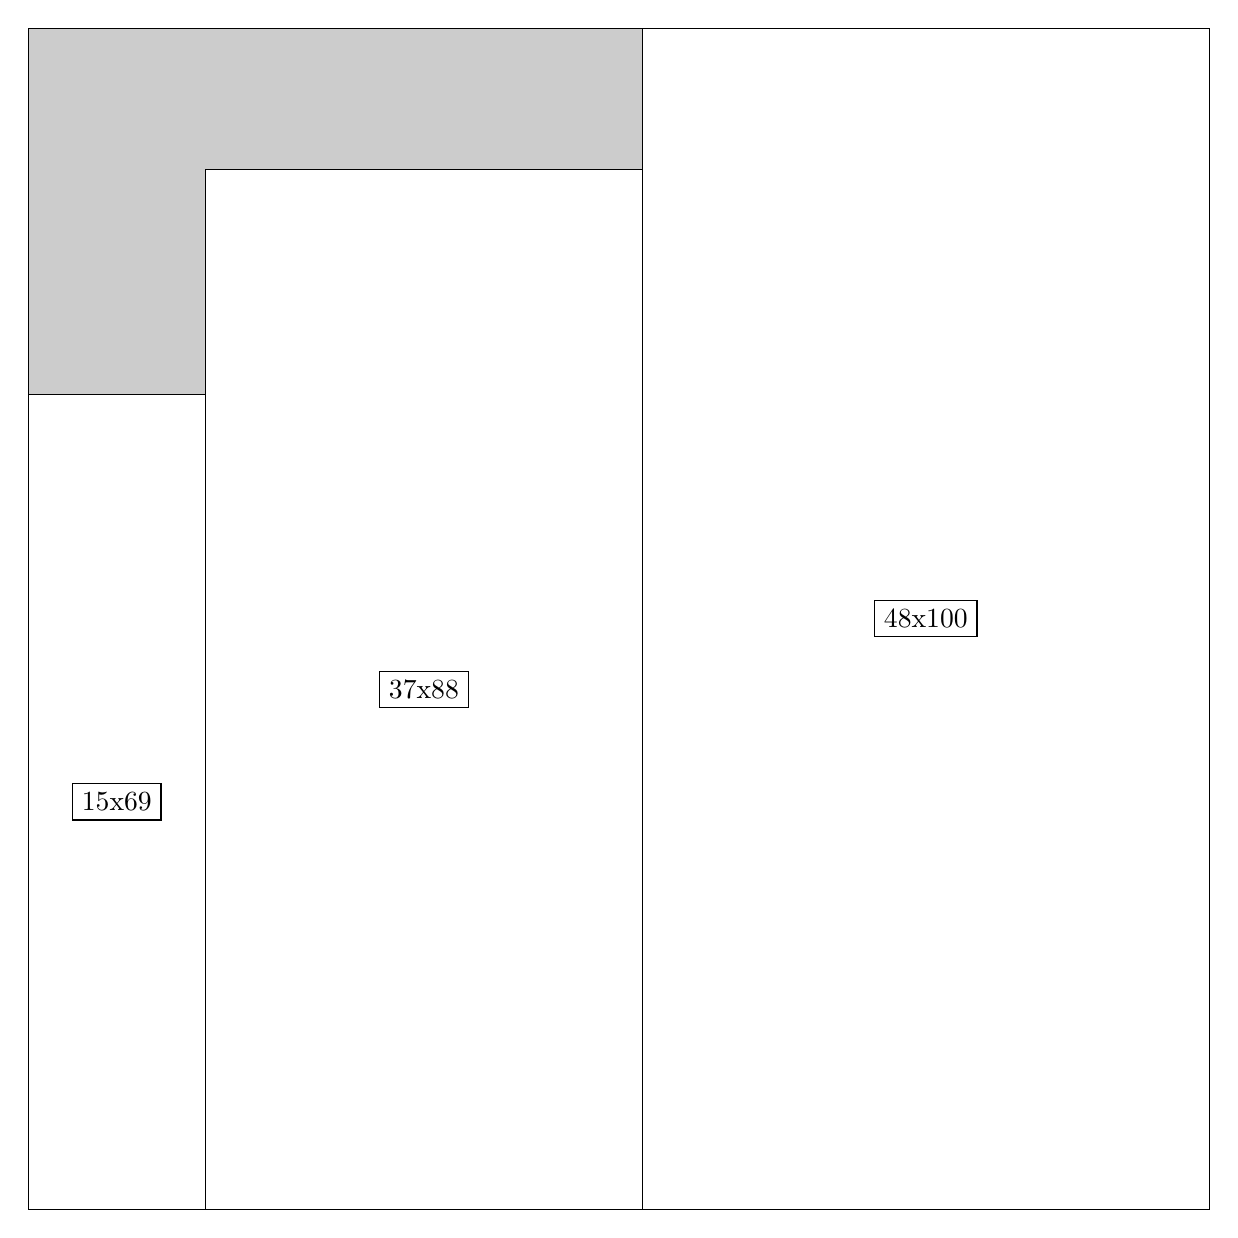
\begin{tikzpicture}[shorten >=1pt,scale=1.0,every node/.style={scale=1.0},->]
\tikzstyle{vertex}=[circle,fill=black!25,minimum size=14pt,inner sep=0pt]
\filldraw[fill=gray!40!white, draw=black] (0,0) rectangle (15.0,15.0);
\foreach \name/\x/\y/\w/\h in {48x100/7.8/0.0/7.199999999999999/15.0,37x88/2.25/0.0/5.55/13.2,15x69/0.0/0.0/2.25/10.35}
\filldraw[fill=white!40!white, draw=black] (\x,\y) rectangle node[draw] (\name) {\name} ++(\w,\h);
\end{tikzpicture}


w =48 , h =100 , x =52 , y =0 , v =4800
\par
w =37 , h =88 , x =15 , y =0 , v =3256
\par
w =15 , h =69 , x =0 , y =0 , v =1035
\par
\newpage


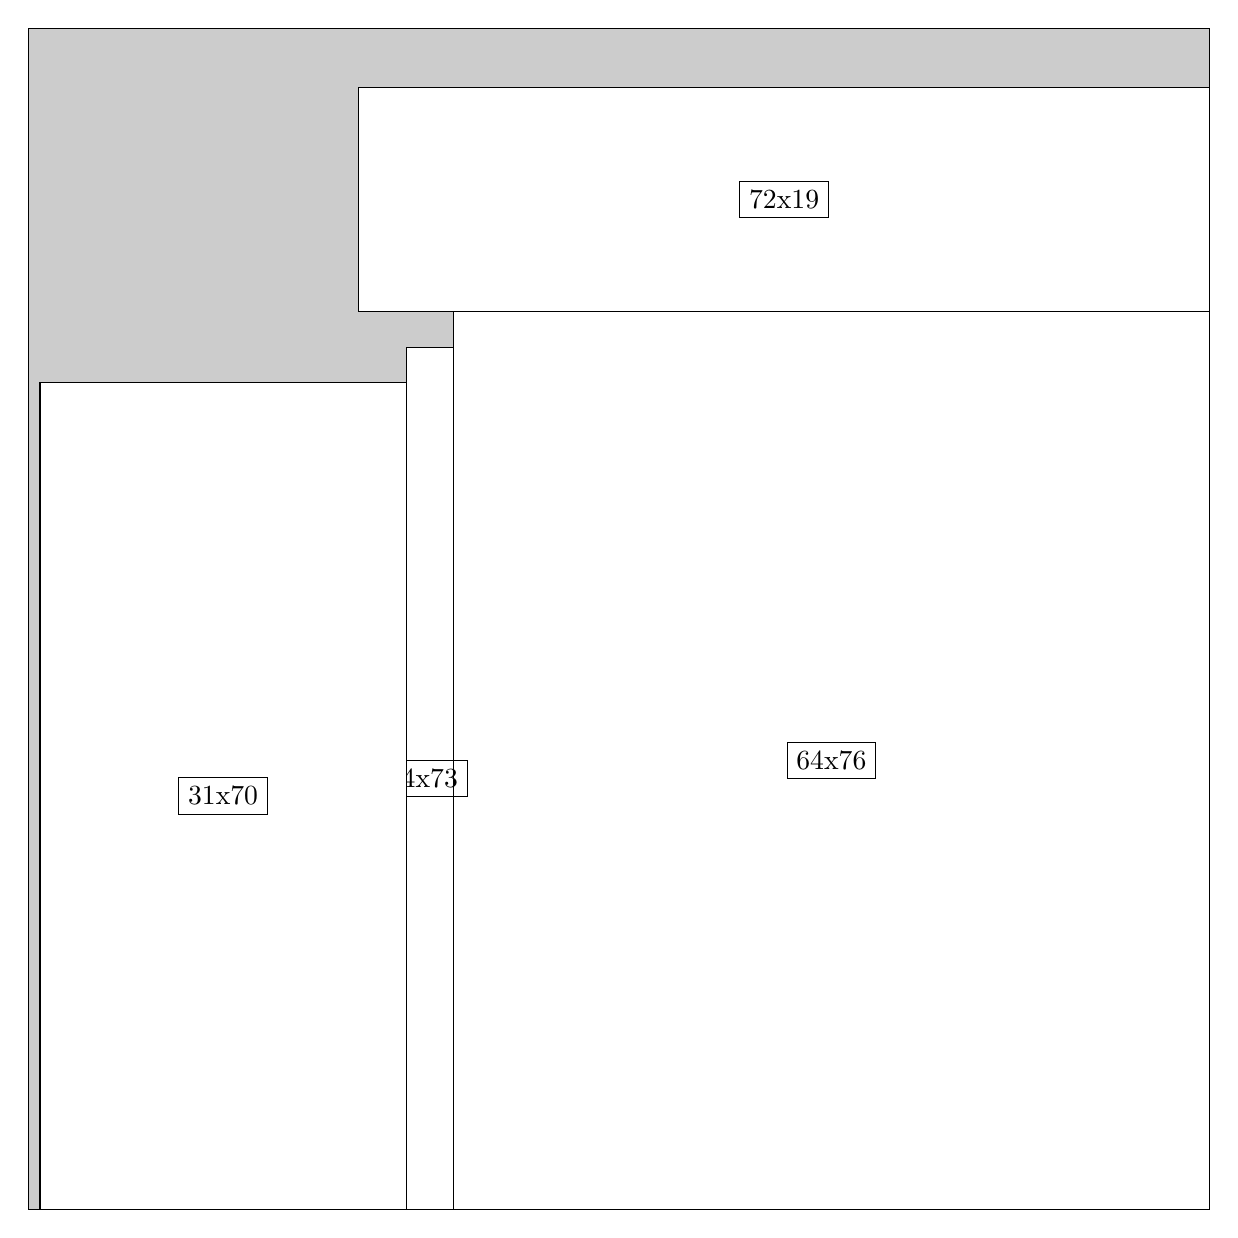
\begin{tikzpicture}[shorten >=1pt,scale=1.0,every node/.style={scale=1.0},->]
\tikzstyle{vertex}=[circle,fill=black!25,minimum size=14pt,inner sep=0pt]
\filldraw[fill=gray!40!white, draw=black] (0,0) rectangle (15.0,15.0);
\foreach \name/\x/\y/\w/\h in {64x76/5.3999999999999995/0.0/9.6/11.4,4x73/4.8/0.0/0.6/10.95,31x70/0.15/0.0/4.6499999999999995/10.5,72x19/4.2/11.4/10.799999999999999/2.85}
\filldraw[fill=white!40!white, draw=black] (\x,\y) rectangle node[draw] (\name) {\name} ++(\w,\h);
\end{tikzpicture}


w =64 , h =76 , x =36 , y =0 , v =4864
\par
w =4 , h =73 , x =32 , y =0 , v =292
\par
w =31 , h =70 , x =1 , y =0 , v =2170
\par
w =72 , h =19 , x =28 , y =76 , v =1368
\par
\newpage


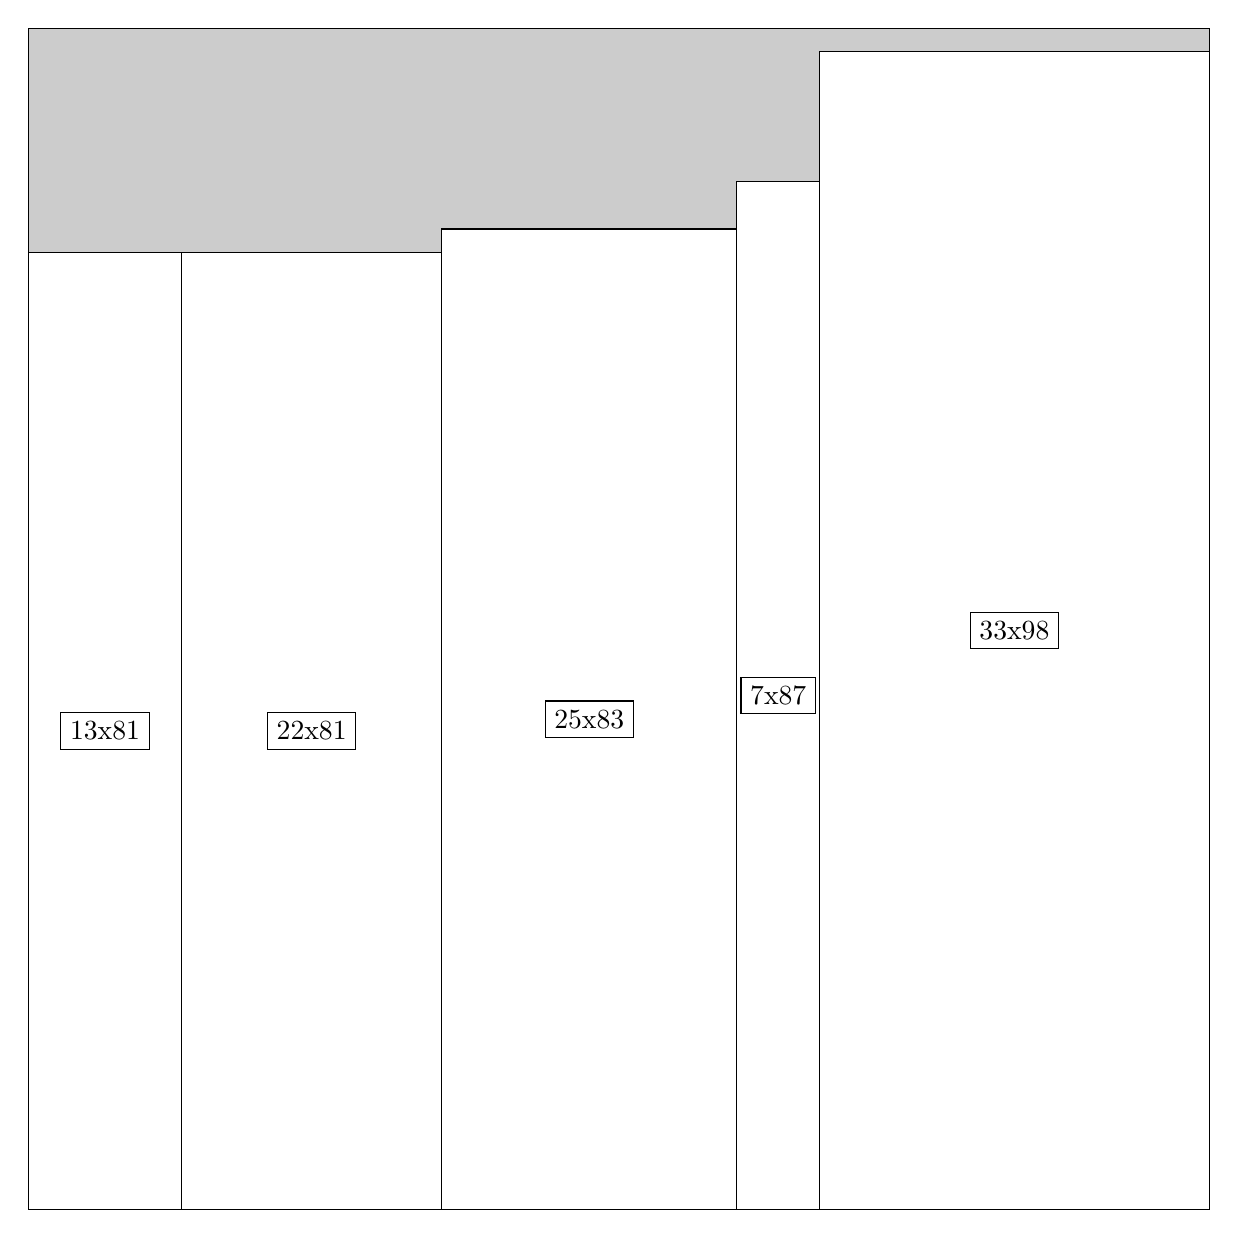
\begin{tikzpicture}[shorten >=1pt,scale=1.0,every node/.style={scale=1.0},->]
\tikzstyle{vertex}=[circle,fill=black!25,minimum size=14pt,inner sep=0pt]
\filldraw[fill=gray!40!white, draw=black] (0,0) rectangle (15.0,15.0);
\foreach \name/\x/\y/\w/\h in {33x98/10.049999999999999/0.0/4.95/14.7,7x87/9.0/0.0/1.05/13.049999999999999,25x83/5.25/0.0/3.75/12.45,22x81/1.95/0.0/3.3/12.15,13x81/0.0/0.0/1.95/12.15}
\filldraw[fill=white!40!white, draw=black] (\x,\y) rectangle node[draw] (\name) {\name} ++(\w,\h);
\end{tikzpicture}


w =33 , h =98 , x =67 , y =0 , v =3234
\par
w =7 , h =87 , x =60 , y =0 , v =609
\par
w =25 , h =83 , x =35 , y =0 , v =2075
\par
w =22 , h =81 , x =13 , y =0 , v =1782
\par
w =13 , h =81 , x =0 , y =0 , v =1053
\par
\newpage


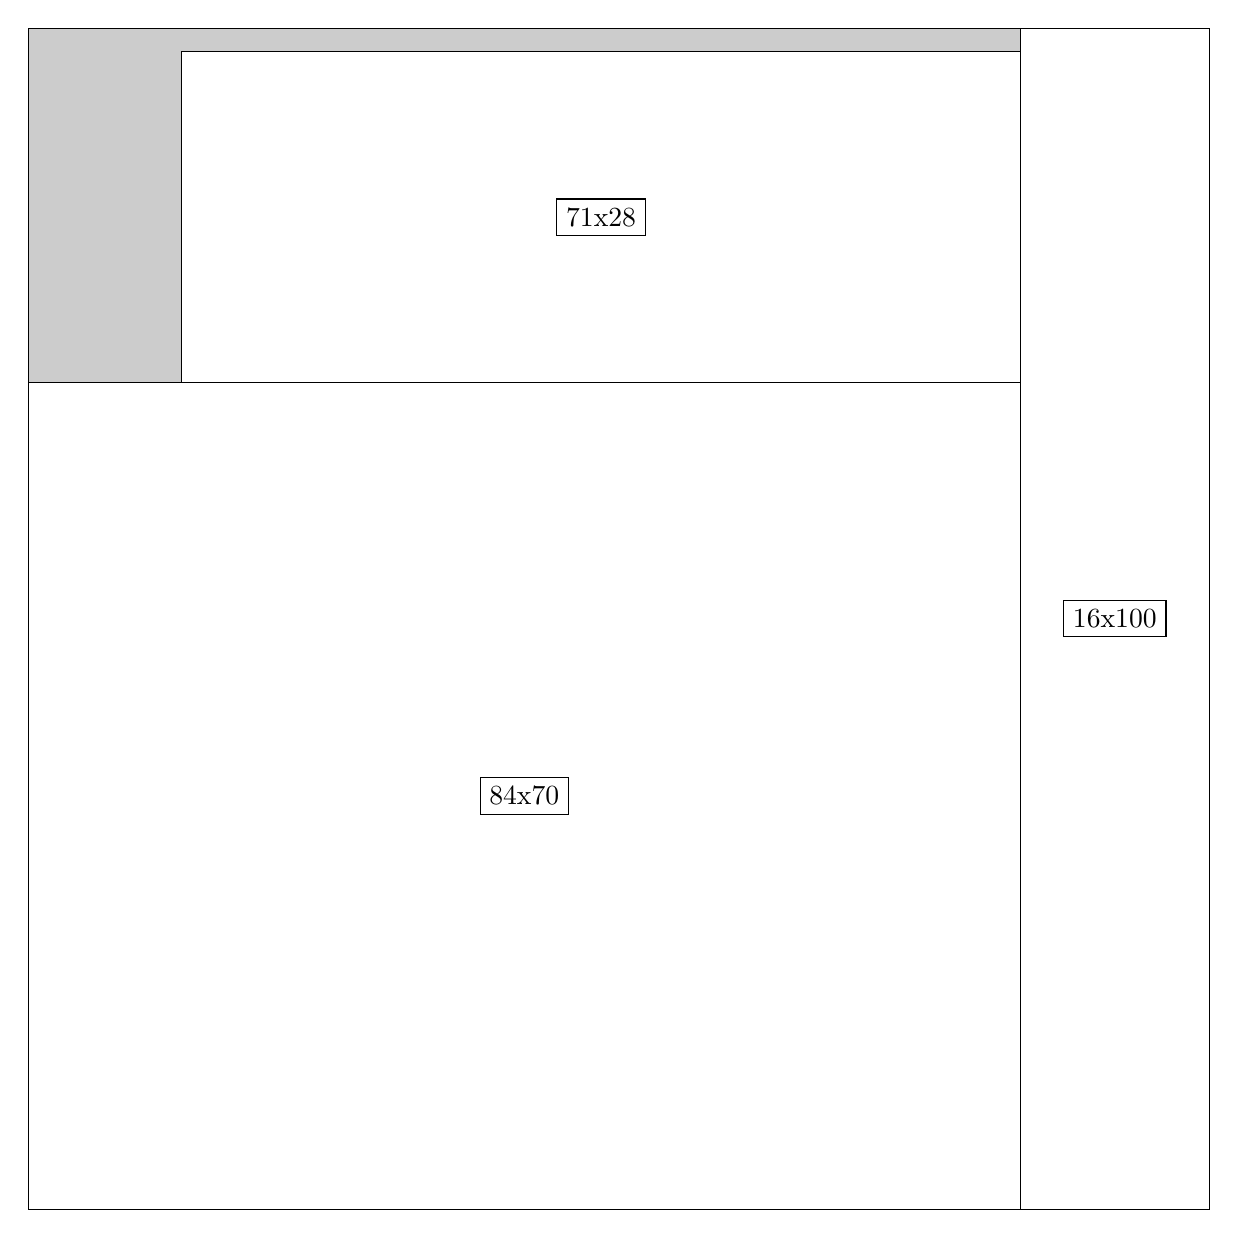
\begin{tikzpicture}[shorten >=1pt,scale=1.0,every node/.style={scale=1.0},->]
\tikzstyle{vertex}=[circle,fill=black!25,minimum size=14pt,inner sep=0pt]
\filldraw[fill=gray!40!white, draw=black] (0,0) rectangle (15.0,15.0);
\foreach \name/\x/\y/\w/\h in {16x100/12.6/0.0/2.4/15.0,84x70/0.0/0.0/12.6/10.5,71x28/1.95/10.5/10.65/4.2}
\filldraw[fill=white!40!white, draw=black] (\x,\y) rectangle node[draw] (\name) {\name} ++(\w,\h);
\end{tikzpicture}


w =16 , h =100 , x =84 , y =0 , v =1600
\par
w =84 , h =70 , x =0 , y =0 , v =5880
\par
w =71 , h =28 , x =13 , y =70 , v =1988
\par
\newpage


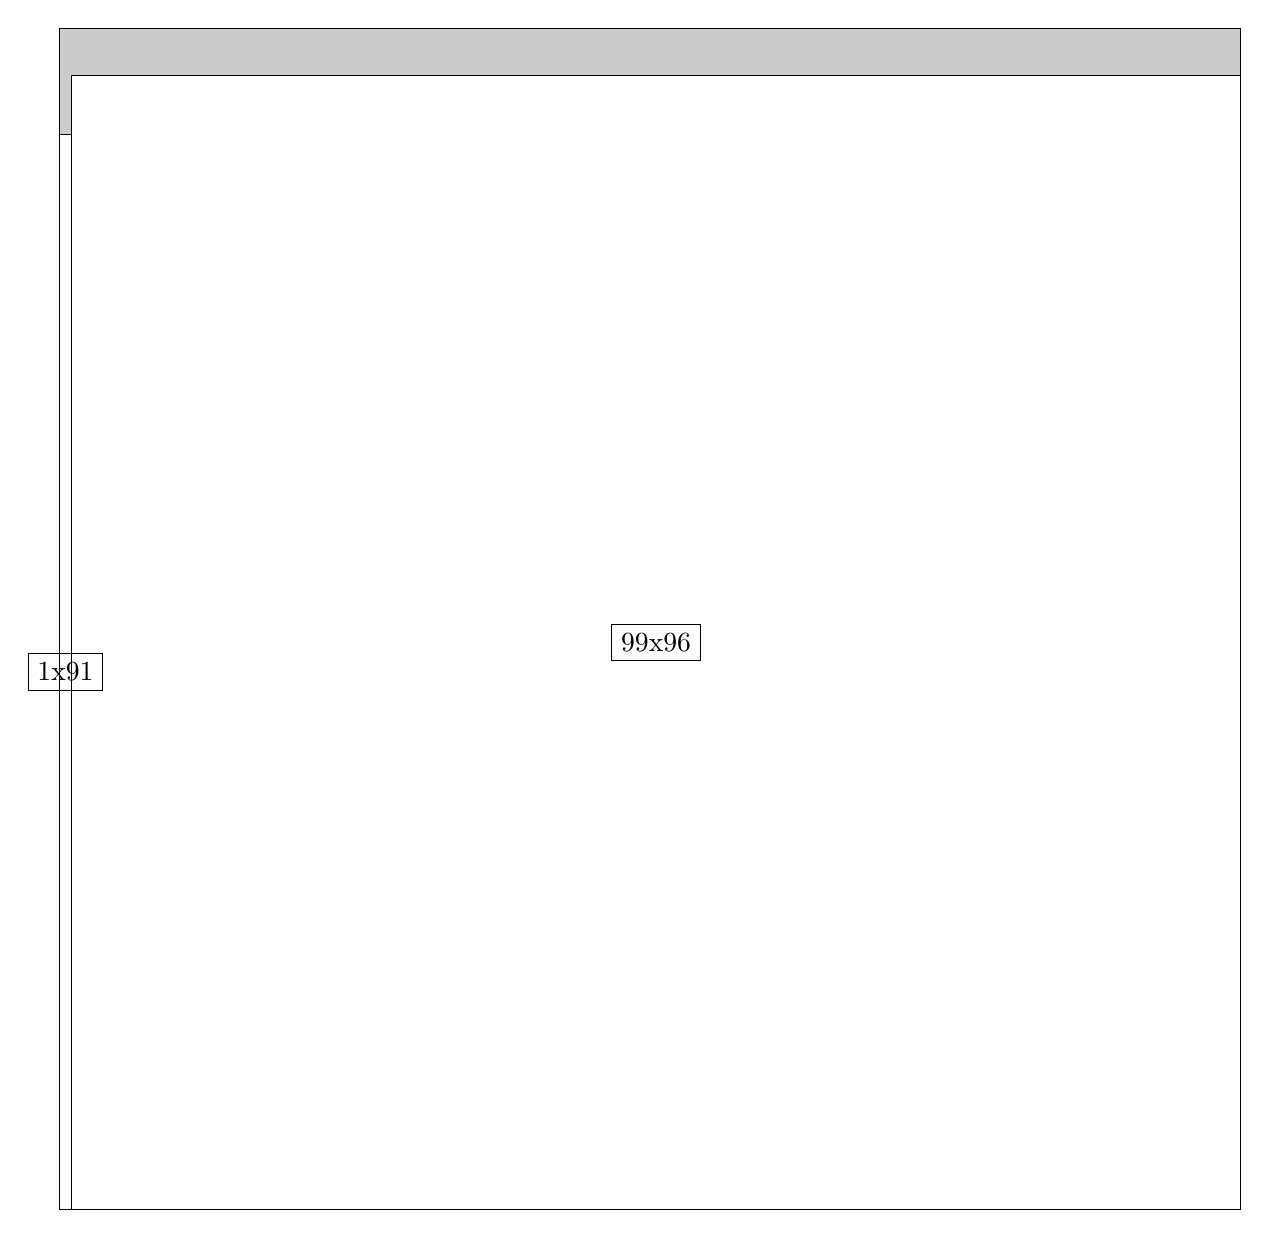
\begin{tikzpicture}[shorten >=1pt,scale=1.0,every node/.style={scale=1.0},->]
\tikzstyle{vertex}=[circle,fill=black!25,minimum size=14pt,inner sep=0pt]
\filldraw[fill=gray!40!white, draw=black] (0,0) rectangle (15.0,15.0);
\foreach \name/\x/\y/\w/\h in {99x96/0.15/0.0/14.85/14.399999999999999,1x91/0.0/0.0/0.15/13.65}
\filldraw[fill=white!40!white, draw=black] (\x,\y) rectangle node[draw] (\name) {\name} ++(\w,\h);
\end{tikzpicture}


w =99 , h =96 , x =1 , y =0 , v =9504
\par
w =1 , h =91 , x =0 , y =0 , v =91
\par
\newpage


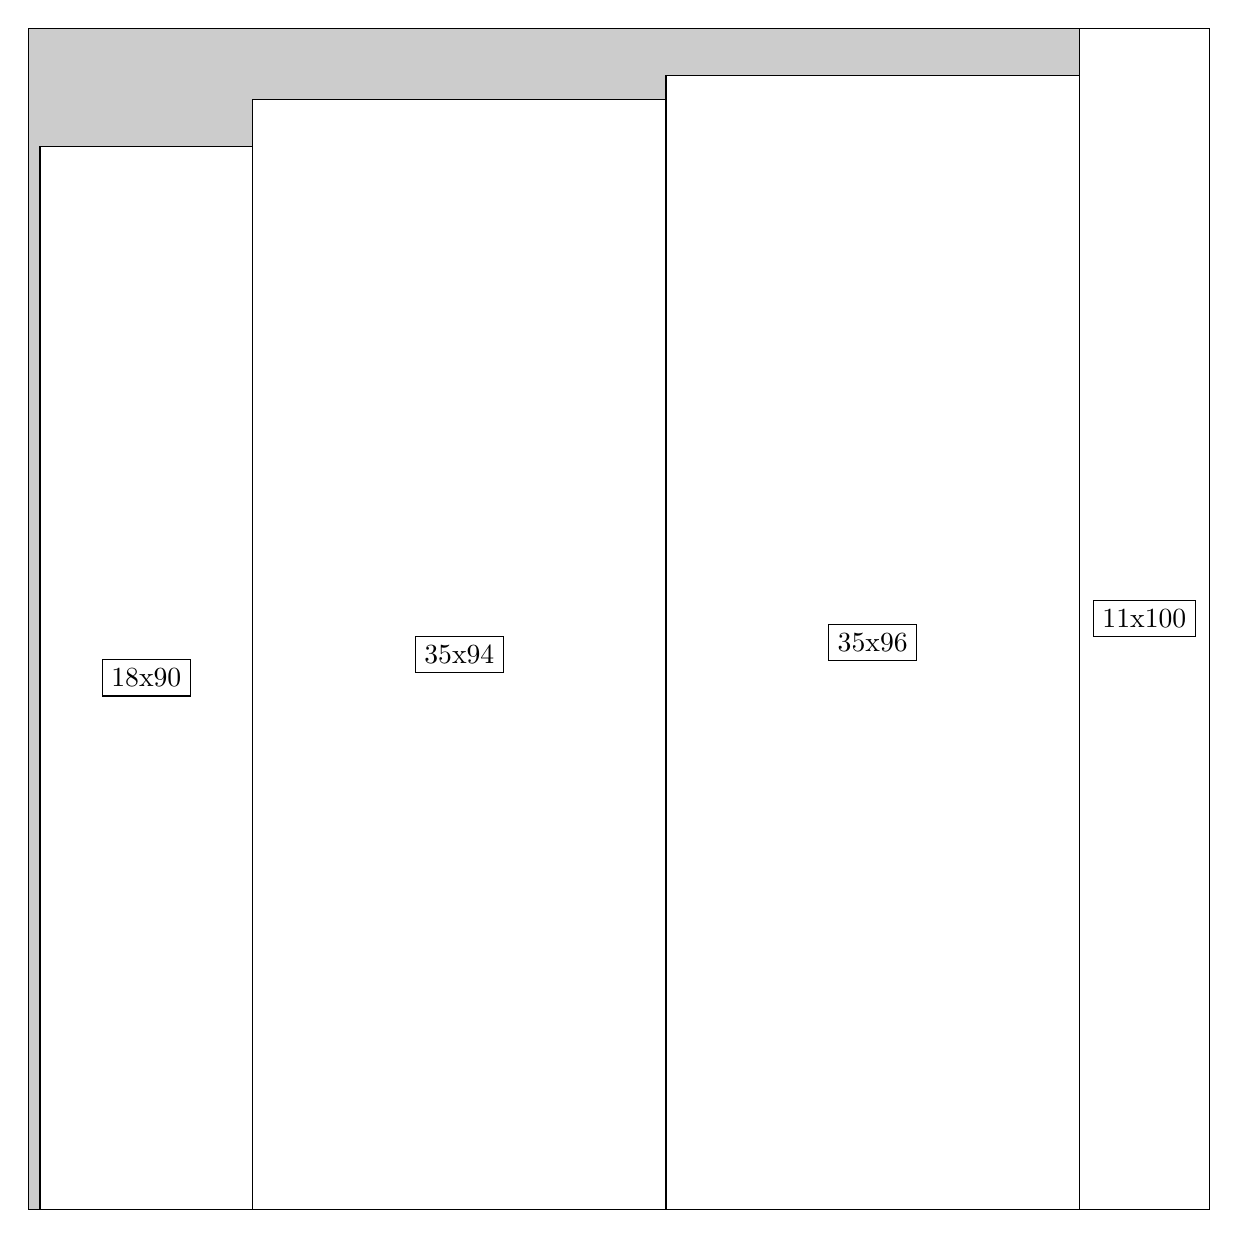
\begin{tikzpicture}[shorten >=1pt,scale=1.0,every node/.style={scale=1.0},->]
\tikzstyle{vertex}=[circle,fill=black!25,minimum size=14pt,inner sep=0pt]
\filldraw[fill=gray!40!white, draw=black] (0,0) rectangle (15.0,15.0);
\foreach \name/\x/\y/\w/\h in {11x100/13.35/0.0/1.65/15.0,35x96/8.1/0.0/5.25/14.399999999999999,35x94/2.85/0.0/5.25/14.1,18x90/0.15/0.0/2.6999999999999997/13.5}
\filldraw[fill=white!40!white, draw=black] (\x,\y) rectangle node[draw] (\name) {\name} ++(\w,\h);
\end{tikzpicture}


w =11 , h =100 , x =89 , y =0 , v =1100
\par
w =35 , h =96 , x =54 , y =0 , v =3360
\par
w =35 , h =94 , x =19 , y =0 , v =3290
\par
w =18 , h =90 , x =1 , y =0 , v =1620
\par
\newpage


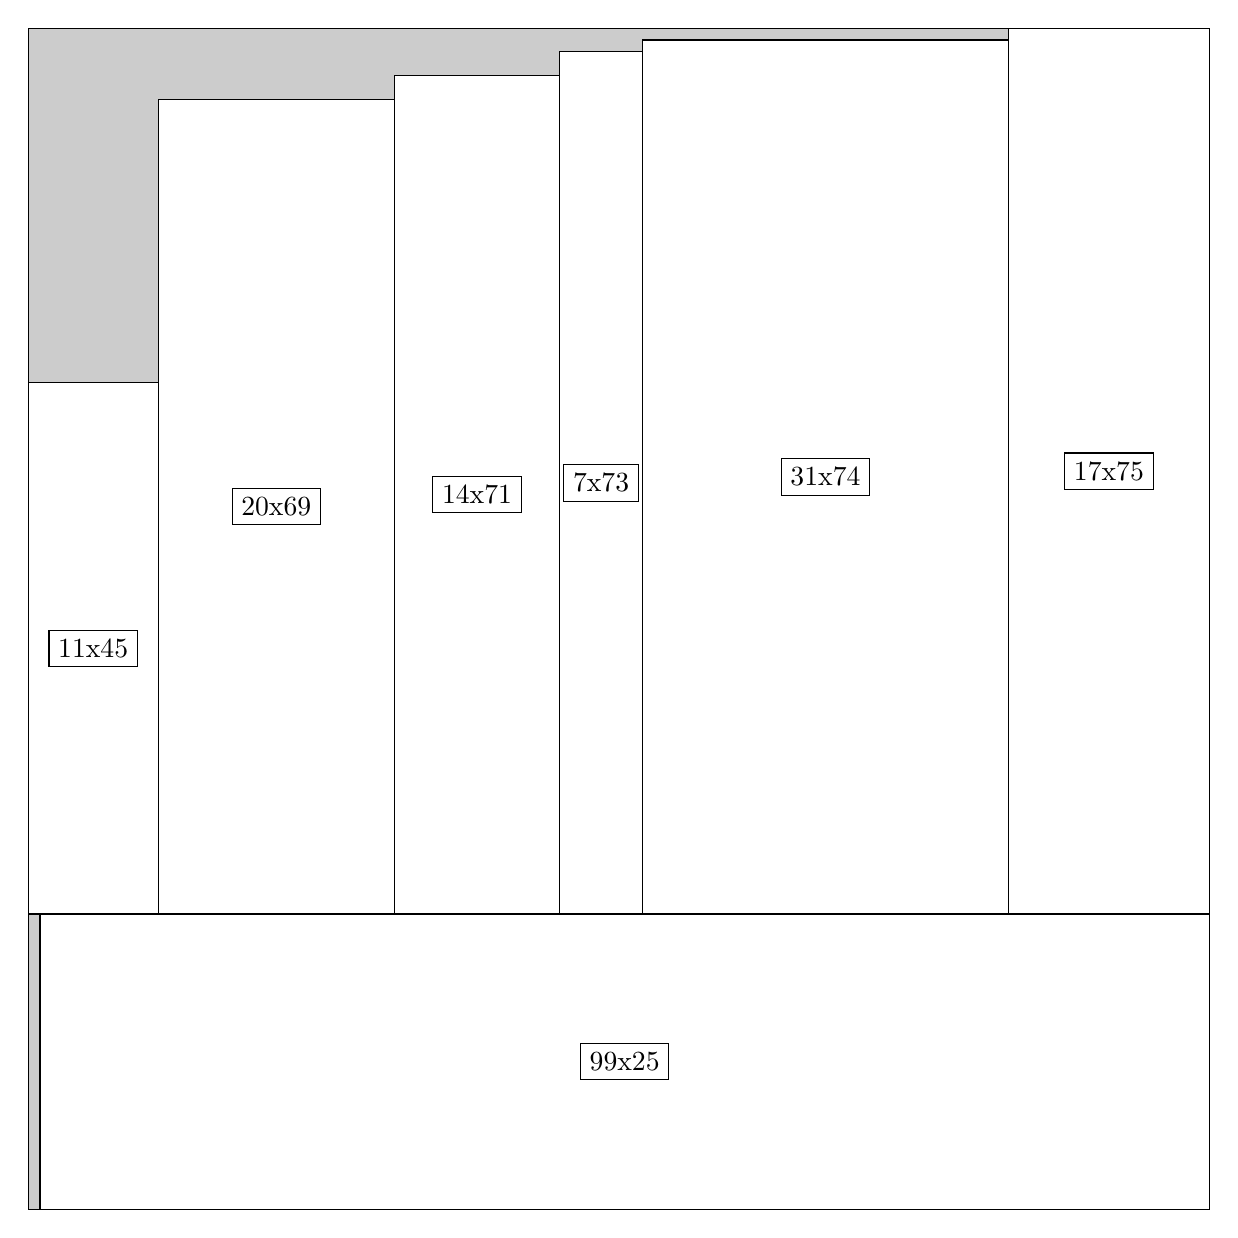
\begin{tikzpicture}[shorten >=1pt,scale=1.0,every node/.style={scale=1.0},->]
\tikzstyle{vertex}=[circle,fill=black!25,minimum size=14pt,inner sep=0pt]
\filldraw[fill=gray!40!white, draw=black] (0,0) rectangle (15.0,15.0);
\foreach \name/\x/\y/\w/\h in {99x25/0.15/0.0/14.85/3.75,17x75/12.45/3.75/2.55/11.25,31x74/7.8/3.75/4.6499999999999995/11.1,7x73/6.75/3.75/1.05/10.95,14x71/4.6499999999999995/3.75/2.1/10.65,20x69/1.65/3.75/3.0/10.35,11x45/0.0/3.75/1.65/6.75}
\filldraw[fill=white!40!white, draw=black] (\x,\y) rectangle node[draw] (\name) {\name} ++(\w,\h);
\end{tikzpicture}


w =99 , h =25 , x =1 , y =0 , v =2475
\par
w =17 , h =75 , x =83 , y =25 , v =1275
\par
w =31 , h =74 , x =52 , y =25 , v =2294
\par
w =7 , h =73 , x =45 , y =25 , v =511
\par
w =14 , h =71 , x =31 , y =25 , v =994
\par
w =20 , h =69 , x =11 , y =25 , v =1380
\par
w =11 , h =45 , x =0 , y =25 , v =495
\par
\newpage


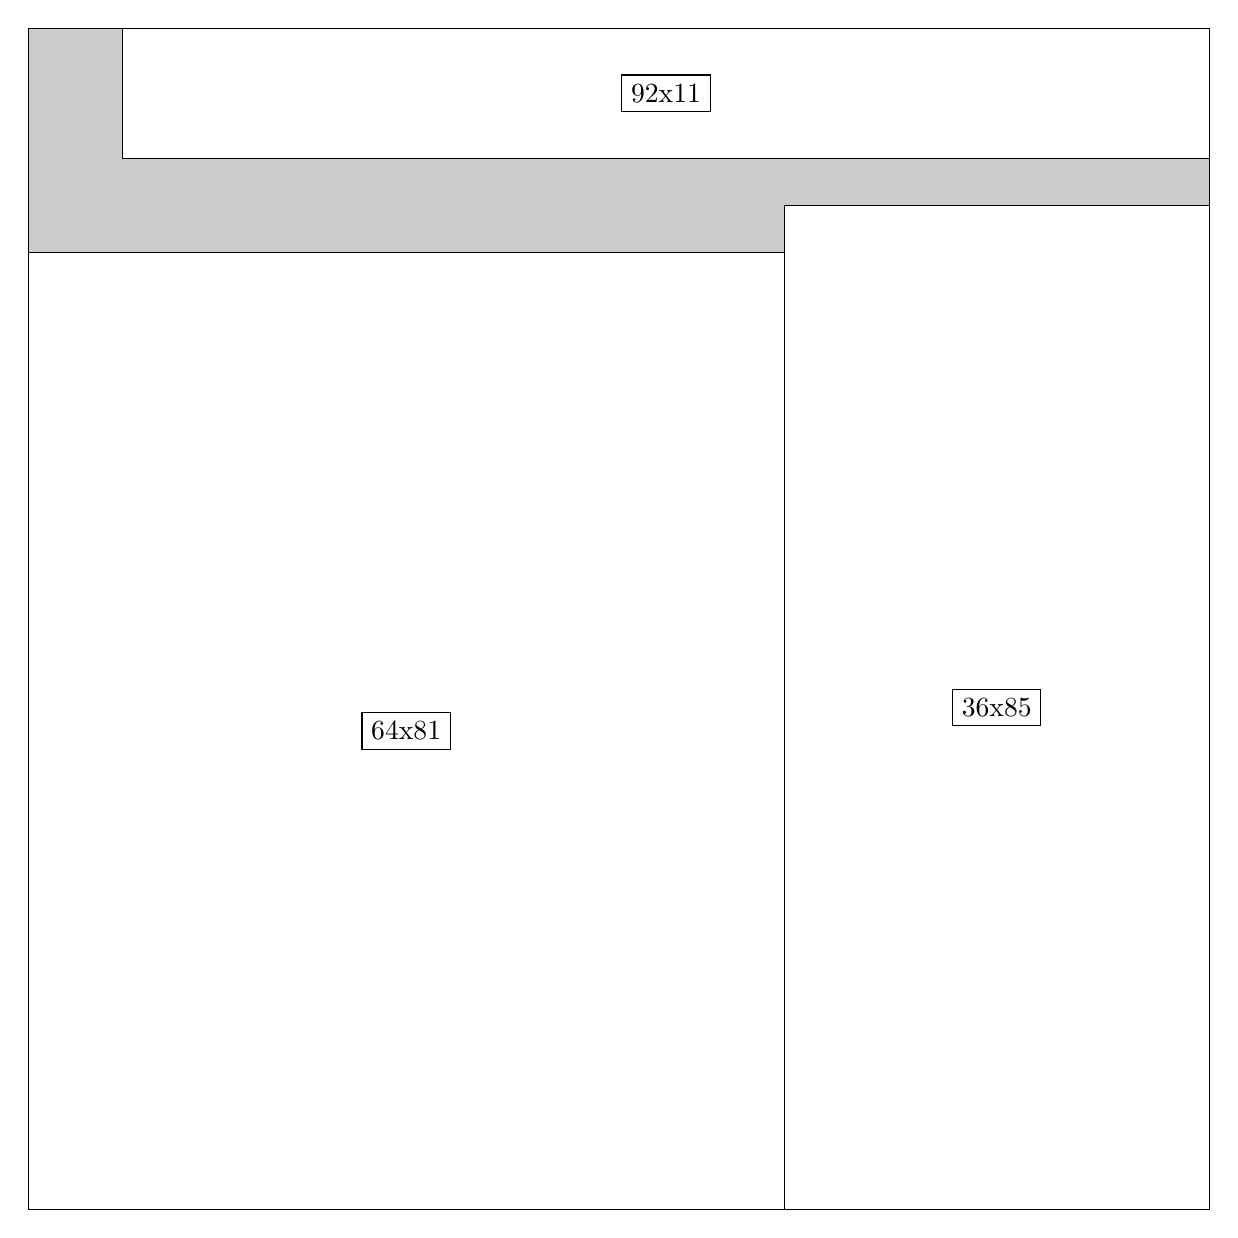
\begin{tikzpicture}[shorten >=1pt,scale=1.0,every node/.style={scale=1.0},->]
\tikzstyle{vertex}=[circle,fill=black!25,minimum size=14pt,inner sep=0pt]
\filldraw[fill=gray!40!white, draw=black] (0,0) rectangle (15.0,15.0);
\foreach \name/\x/\y/\w/\h in {36x85/9.6/0.0/5.3999999999999995/12.75,64x81/0.0/0.0/9.6/12.15,92x11/1.2/13.35/13.799999999999999/1.65}
\filldraw[fill=white!40!white, draw=black] (\x,\y) rectangle node[draw] (\name) {\name} ++(\w,\h);
\end{tikzpicture}


w =36 , h =85 , x =64 , y =0 , v =3060
\par
w =64 , h =81 , x =0 , y =0 , v =5184
\par
w =92 , h =11 , x =8 , y =89 , v =1012
\par
\newpage


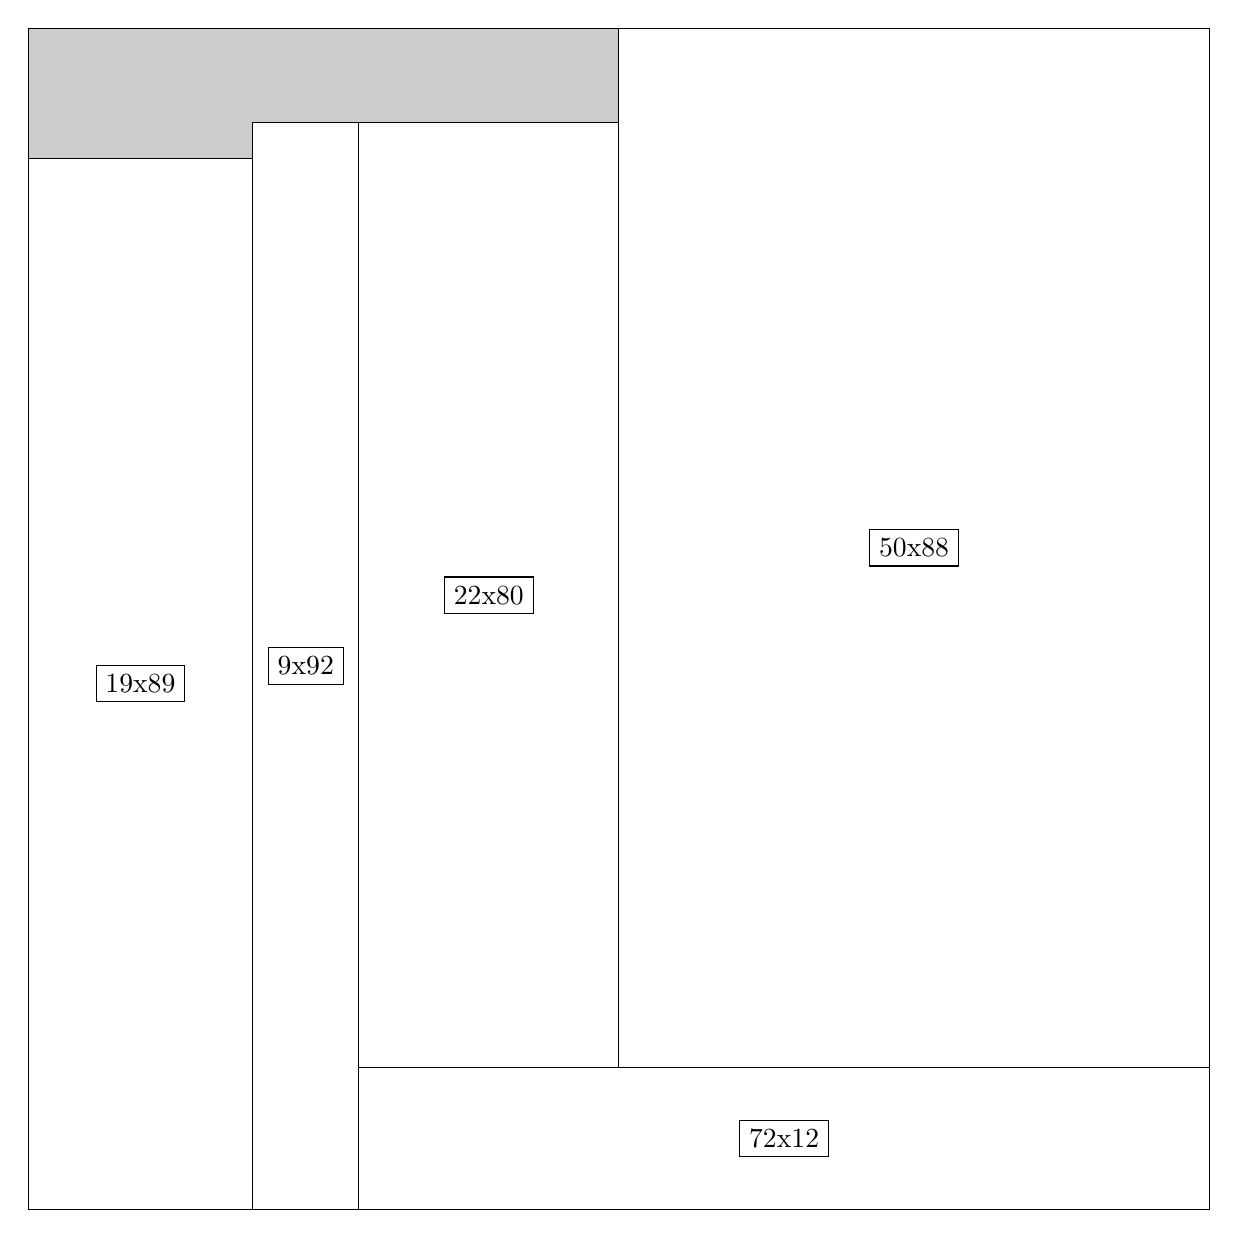
\begin{tikzpicture}[shorten >=1pt,scale=1.0,every node/.style={scale=1.0},->]
\tikzstyle{vertex}=[circle,fill=black!25,minimum size=14pt,inner sep=0pt]
\filldraw[fill=gray!40!white, draw=black] (0,0) rectangle (15.0,15.0);
\foreach \name/\x/\y/\w/\h in {72x12/4.2/0.0/10.799999999999999/1.7999999999999998,50x88/7.5/1.7999999999999998/7.5/13.2,22x80/4.2/1.7999999999999998/3.3/12.0,9x92/2.85/0.0/1.3499999999999999/13.799999999999999,19x89/0.0/0.0/2.85/13.35}
\filldraw[fill=white!40!white, draw=black] (\x,\y) rectangle node[draw] (\name) {\name} ++(\w,\h);
\end{tikzpicture}


w =72 , h =12 , x =28 , y =0 , v =864
\par
w =50 , h =88 , x =50 , y =12 , v =4400
\par
w =22 , h =80 , x =28 , y =12 , v =1760
\par
w =9 , h =92 , x =19 , y =0 , v =828
\par
w =19 , h =89 , x =0 , y =0 , v =1691
\par
\newpage


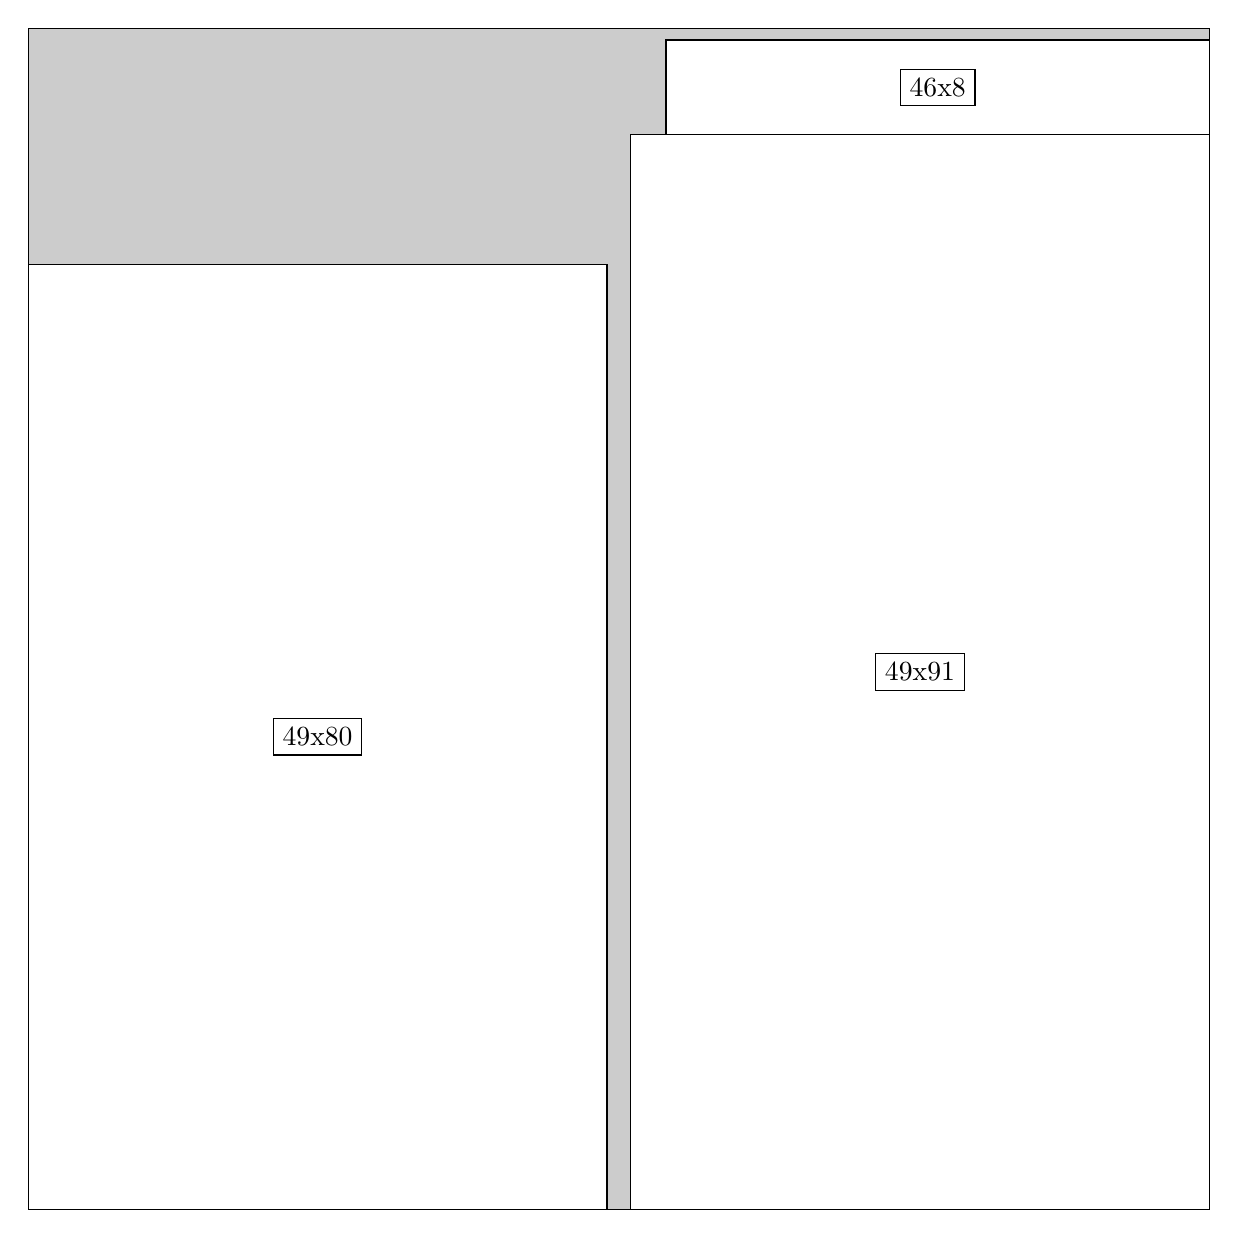
\begin{tikzpicture}[shorten >=1pt,scale=1.0,every node/.style={scale=1.0},->]
\tikzstyle{vertex}=[circle,fill=black!25,minimum size=14pt,inner sep=0pt]
\filldraw[fill=gray!40!white, draw=black] (0,0) rectangle (15.0,15.0);
\foreach \name/\x/\y/\w/\h in {49x91/7.6499999999999995/0.0/7.35/13.65,46x8/8.1/13.65/6.8999999999999995/1.2,49x80/0.0/0.0/7.35/12.0}
\filldraw[fill=white!40!white, draw=black] (\x,\y) rectangle node[draw] (\name) {\name} ++(\w,\h);
\end{tikzpicture}


w =49 , h =91 , x =51 , y =0 , v =4459
\par
w =46 , h =8 , x =54 , y =91 , v =368
\par
w =49 , h =80 , x =0 , y =0 , v =3920
\par
\newpage


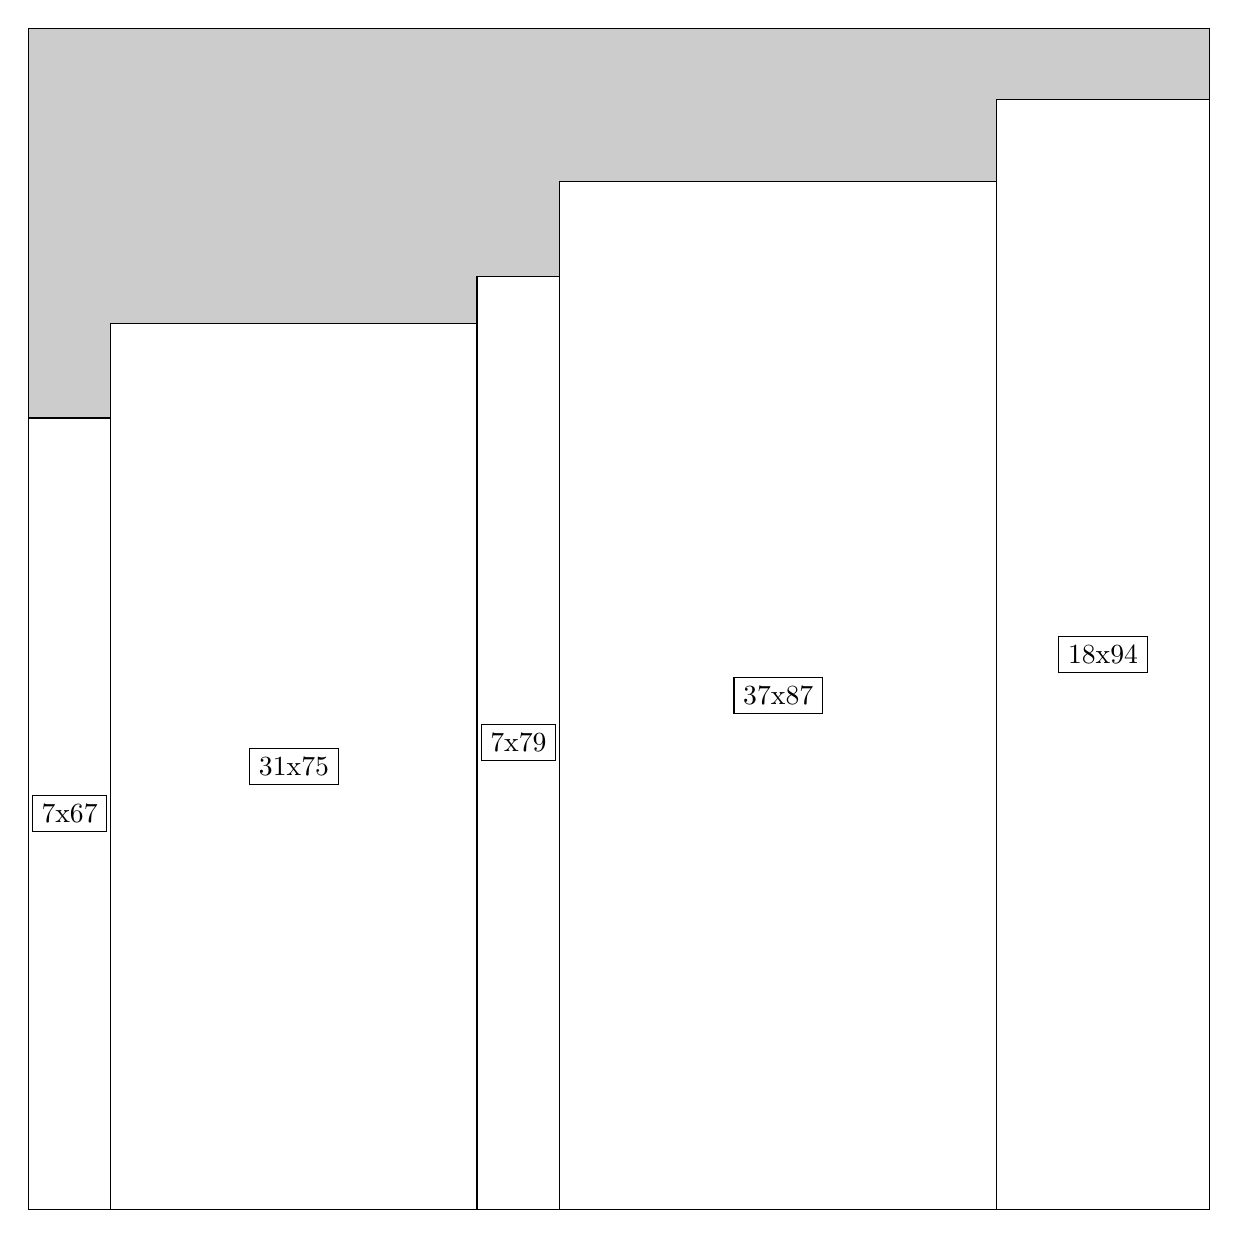
\begin{tikzpicture}[shorten >=1pt,scale=1.0,every node/.style={scale=1.0},->]
\tikzstyle{vertex}=[circle,fill=black!25,minimum size=14pt,inner sep=0pt]
\filldraw[fill=gray!40!white, draw=black] (0,0) rectangle (15.0,15.0);
\foreach \name/\x/\y/\w/\h in {18x94/12.299999999999999/0.0/2.6999999999999997/14.1,37x87/6.75/0.0/5.55/13.049999999999999,7x79/5.7/0.0/1.05/11.85,31x75/1.05/0.0/4.6499999999999995/11.25,7x67/0.0/0.0/1.05/10.049999999999999}
\filldraw[fill=white!40!white, draw=black] (\x,\y) rectangle node[draw] (\name) {\name} ++(\w,\h);
\end{tikzpicture}


w =18 , h =94 , x =82 , y =0 , v =1692
\par
w =37 , h =87 , x =45 , y =0 , v =3219
\par
w =7 , h =79 , x =38 , y =0 , v =553
\par
w =31 , h =75 , x =7 , y =0 , v =2325
\par
w =7 , h =67 , x =0 , y =0 , v =469
\par
\newpage


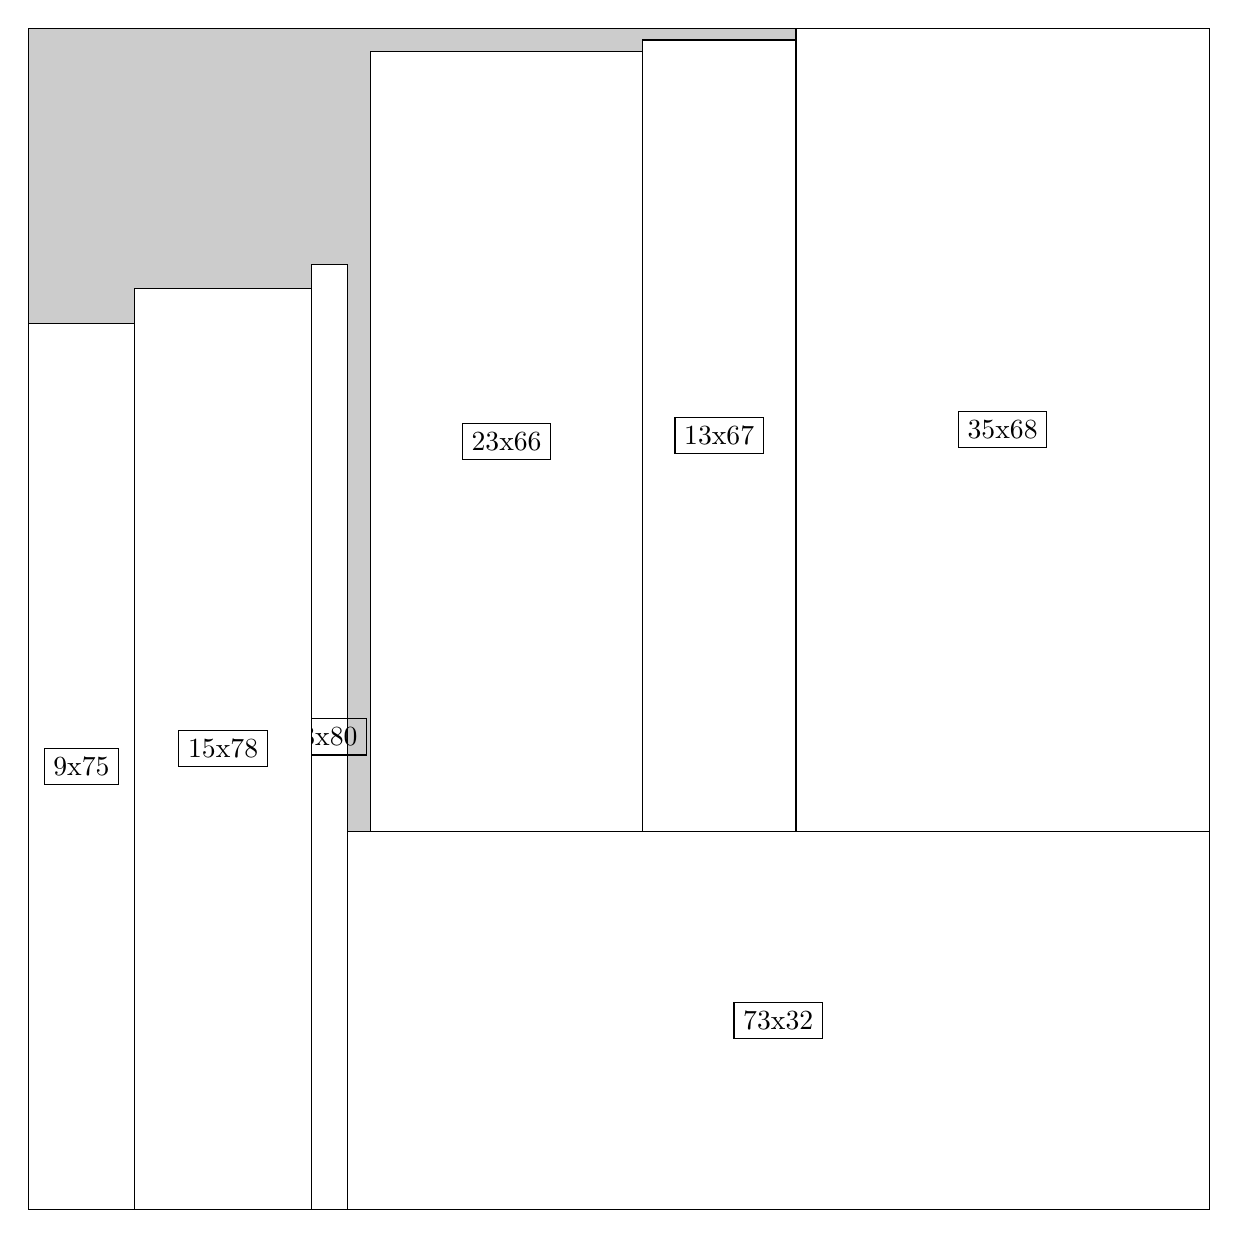
\begin{tikzpicture}[shorten >=1pt,scale=1.0,every node/.style={scale=1.0},->]
\tikzstyle{vertex}=[circle,fill=black!25,minimum size=14pt,inner sep=0pt]
\filldraw[fill=gray!40!white, draw=black] (0,0) rectangle (15.0,15.0);
\foreach \name/\x/\y/\w/\h in {73x32/4.05/0.0/10.95/4.8,35x68/9.75/4.8/5.25/10.2,13x67/7.8/4.8/1.95/10.049999999999999,23x66/4.35/4.8/3.4499999999999997/9.9,3x80/3.5999999999999996/0.0/0.44999999999999996/12.0,15x78/1.3499999999999999/0.0/2.25/11.7,9x75/0.0/0.0/1.3499999999999999/11.25}
\filldraw[fill=white!40!white, draw=black] (\x,\y) rectangle node[draw] (\name) {\name} ++(\w,\h);
\end{tikzpicture}


w =73 , h =32 , x =27 , y =0 , v =2336
\par
w =35 , h =68 , x =65 , y =32 , v =2380
\par
w =13 , h =67 , x =52 , y =32 , v =871
\par
w =23 , h =66 , x =29 , y =32 , v =1518
\par
w =3 , h =80 , x =24 , y =0 , v =240
\par
w =15 , h =78 , x =9 , y =0 , v =1170
\par
w =9 , h =75 , x =0 , y =0 , v =675
\par
\newpage


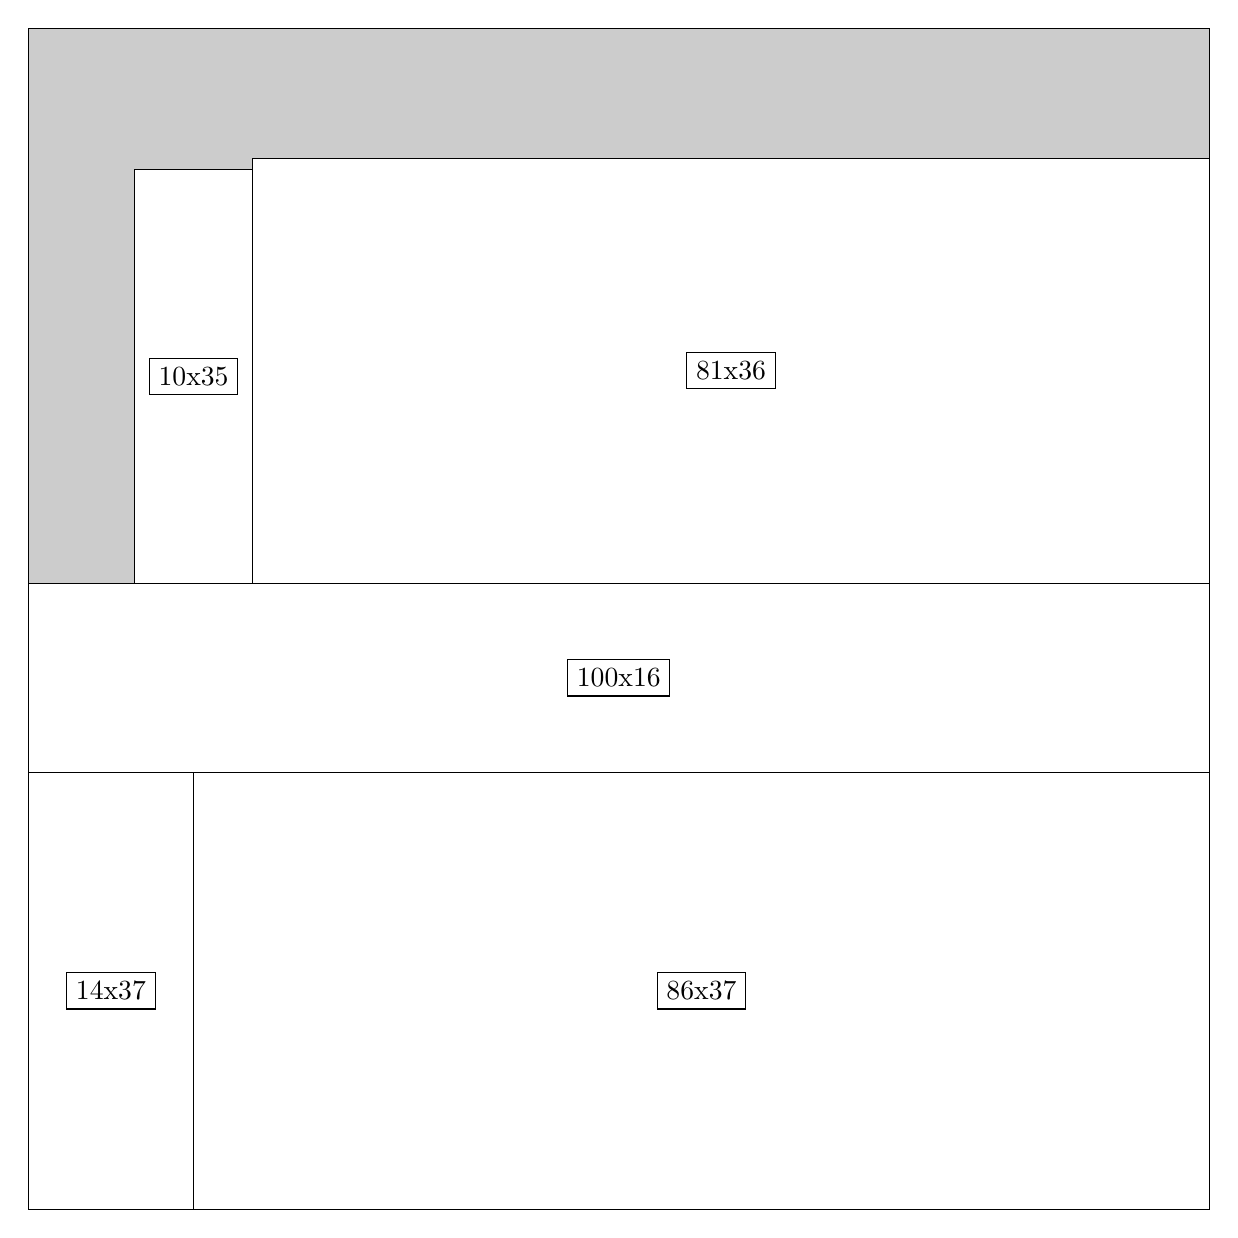
\begin{tikzpicture}[shorten >=1pt,scale=1.0,every node/.style={scale=1.0},->]
\tikzstyle{vertex}=[circle,fill=black!25,minimum size=14pt,inner sep=0pt]
\filldraw[fill=gray!40!white, draw=black] (0,0) rectangle (15.0,15.0);
\foreach \name/\x/\y/\w/\h in {86x37/2.1/0.0/12.9/5.55,14x37/0.0/0.0/2.1/5.55,100x16/0.0/5.55/15.0/2.4,81x36/2.85/7.949999999999999/12.15/5.3999999999999995,10x35/1.3499999999999999/7.949999999999999/1.5/5.25}
\filldraw[fill=white!40!white, draw=black] (\x,\y) rectangle node[draw] (\name) {\name} ++(\w,\h);
\end{tikzpicture}


w =86 , h =37 , x =14 , y =0 , v =3182
\par
w =14 , h =37 , x =0 , y =0 , v =518
\par
w =100 , h =16 , x =0 , y =37 , v =1600
\par
w =81 , h =36 , x =19 , y =53 , v =2916
\par
w =10 , h =35 , x =9 , y =53 , v =350
\par
\newpage


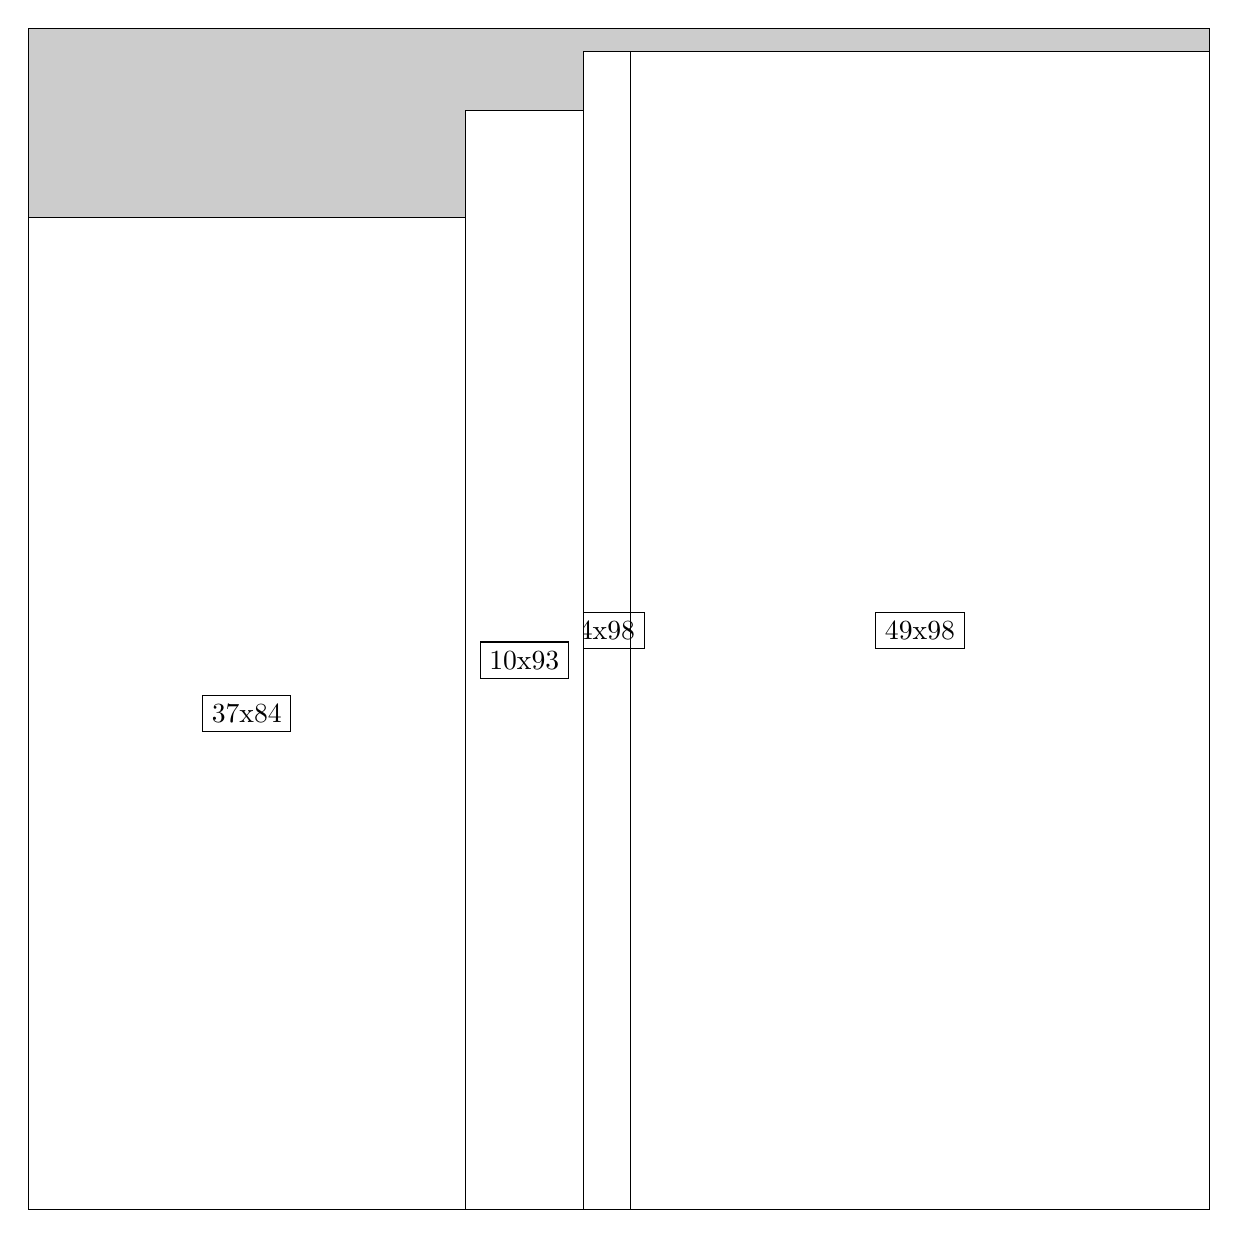
\begin{tikzpicture}[shorten >=1pt,scale=1.0,every node/.style={scale=1.0},->]
\tikzstyle{vertex}=[circle,fill=black!25,minimum size=14pt,inner sep=0pt]
\filldraw[fill=gray!40!white, draw=black] (0,0) rectangle (15.0,15.0);
\foreach \name/\x/\y/\w/\h in {49x98/7.6499999999999995/0.0/7.35/14.7,4x98/7.05/0.0/0.6/14.7,10x93/5.55/0.0/1.5/13.95,37x84/0.0/0.0/5.55/12.6}
\filldraw[fill=white!40!white, draw=black] (\x,\y) rectangle node[draw] (\name) {\name} ++(\w,\h);
\end{tikzpicture}


w =49 , h =98 , x =51 , y =0 , v =4802
\par
w =4 , h =98 , x =47 , y =0 , v =392
\par
w =10 , h =93 , x =37 , y =0 , v =930
\par
w =37 , h =84 , x =0 , y =0 , v =3108
\par
\newpage


\end{document}